
\newcommand{\printfigGraphTypes}{
    \begin{figure}
        \begin{subfigure}{.5\textwidth}
            \centering
            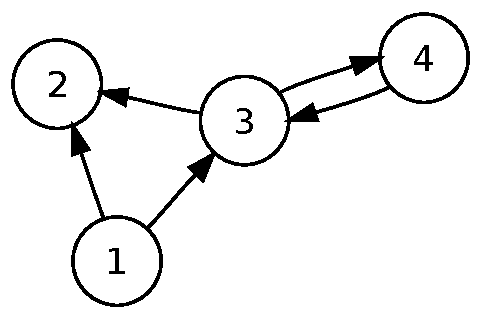
\includegraphics[width=.8\linewidth]{assets/images/Directed_graph_no_background.svg.pdf}
            \caption{Directed graph with cycle between nodes three and four.}
            \label{fig:directedgraph}
        \end{subfigure}
        \begin{subfigure}{.5\textwidth}
            \centering
            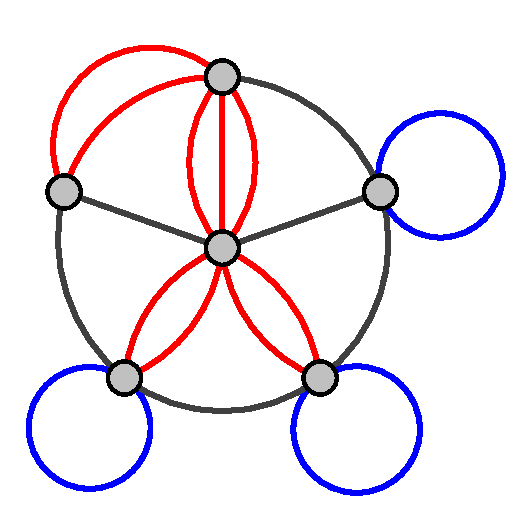
\includegraphics[width=.8\linewidth]{assets/images/Multi-pseudograph.svg.pdf}
            \caption{Multigraph with parallel edges and self-loops}
            \label{fig:multigraph}
        \end{subfigure}%
        \caption[]{Examples of first order graph symantics supported by Jaseci.\footnotemark}
        \label{fig:graph_examples}
    \end{figure}
    \footnotetext{Images credits to wiki contributers~\cite{wiki:Directed_graph_no_background.svg,wiki:Multi-pseudograph.svg}}
}


\newcommand{\printfigHelloWorldBaby}{
    \begin{figure}%{r}{0.5\textwidth}
        \centering
        
\includegraphics[width=.3\linewidth]{assets/images/hello_world_baby.jpg}
        \caption[]{World's youngest coder with valid HTML on shirt.\footnotemark}
        \label{fig:hello_baby}
    \end{figure}
    \footnotetext{Image credit to wiki contributer~\cite{wiki:hello_world_baby.jpg}}
}

\newcommand{\printtabPrecedence}{
    \begin{table}[t]
        \footnotesize
        \centering
        \begin{tabular}{l l l}
            \toprule
            \textbf{Rank} & \textbf{Symbol}                            & \textbf{Description}                           \\
            \midrule
            1             & \texttt{( ), [ ], ., ::, spawn}            & Parenthetical/grouping, node/edge manipulation \\
            2             & \texttt{\textasciicircum, []}              & Exponent,  Index                               \\
            3             & \texttt{*, /, \%  }                        & Multiplication, division, modulo               \\
            4             & \texttt{+, -}                              & Addition, subtraction                          \\
            5             & \texttt{==, !=, >=, <=, >, <, in, not in } & Comparison                                     \\
            6             & \texttt{\&\&, ||, and, or  }               & Logical                                        \\
            7             & \texttt{-->, <--, -[]->, <-[]-}            & Connect                                        \\
            8             & \texttt{=, +=, -=, *=, /=, := }            & Assignment                                     \\
            \bottomrule
        \end{tabular}
        \caption{Precedence of operations in Jac}
        \label{tab:jacprecedence} % Unique label used for referencing the table in-text
        %\addcontentsline{toc}{table}{Table \ref{tab:jacprecedence}} % Uncomment to add the table to the table of contents
    \end{table}
}

\newcommand{\printtabStrOps}{
    \begin{table}[t]
        \footnotesize
        \centering
        \rowcolors{1}{light-cyan}{light-gray}
        \begin{tabular}{l p{3cm} p{6cm}}
            \toprule
            \textbf{Op}                                           & \textbf{Args}                                                                                                                                                  & \textbf{Description} \\
            \midrule
            \lstinline{.str::upper}                               & none                                                                                                                                                           &                      \\
            \lstinline{.str::lower}                               & none                                                                                                                                                           &                      \\
            \lstinline{.str::title}                               & none                                                                                                                                                           &                      \\
            \lstinline{.str::capitalize}                          & none                                                                                                                                                           &                      \\
            \lstinline{.str::swap\_case}                          & none                                                                                                                                                           &                      \\
            \lstinline{.str::is\_alnum}                           & none                                                                                                                                                           &                      \\
            \lstinline{.str::is\_digit}                           & none                                                                                                                                                           &                      \\
            \lstinline{.str::is\_title}                           & none                                                                                                                                                           &                      \\
            \lstinline{.str::is\_upper}                           & none                                                                                                                                                           &                      \\
            \lstinline{.str::is\_lower}                           & none                                                                                                                                                           &                      \\
            \lstinline{.str::is\_space}                           & none                                                                                                                                                           &                      \\
            \lstinline{.str::load\_json}                          & none                                                                                                                                                           &                      \\
            \lstinline{.str::count}      & (\textbf{substr}, start, end)            & Returns the number of occurrences of a substring in the given string. Start and end specify range of indices to search                                                                \\
            \lstinline{.str::find}       &   (\textbf{substr}, start, end)            & Returns the index of first occurrence of the substring (if found). If not found, it returns -1. Start and end specify range of indices to search.                                     \\
            \lstinline{.str::split}      & \emph{optional} (separator, maxsplit) & Breaks up a string at the specified separator for maxsplit number of times and returns a list of strings. Default separators is ` ' and maxsplit is unlimited.                        \\
            \lstinline{.str::startswith}                          &                                                                                                                                                                &                      \\
            \lstinline{.str::endswith}                            &                                                                                                                                                                &                      \\
            \lstinline{.str::replace}                             &                                                                                                                                                                &                      \\
            \lstinline{.str::strip}                               & optional,                                                                                                                                                      &                      \\
            \lstinline{.str::lstrip}                              & optional,                                                                                                                                                      &                      \\
            \lstinline{.str::rstrip}                              & optional,                                                                                                                                                      &                      \\
            \bottomrule
        \end{tabular}
        \caption{Complete Library of String Operations}
        \label{tab:strops} % Unique label used for referencing the table in-text
        %\addcontentsline{toc}{table}{Table \ref{tab:jacprecedence}} % Uncomment to add the table to the table of contents
    \end{table}
}

\newcommand{\printtabListOps}{
    \begin{table}[t]
        \footnotesize
        \centering
        \begin{tabular}{l l l}
            \toprule
            \textbf{Op}                     & \textbf{Args} & \textbf{Description} \\
            \midrule
            \lstinline{.list::max}          & none          &                      \\
            \lstinline{.list::min}          & none          &                      \\
            \lstinline{.list::idx\_of\_max} & none          &                      \\
            \lstinline{.list::idx\_of\_min} & none          &                      \\
            \lstinline{.list::copy}         & none          &  Returns a shallow copy of the list  \\
            \lstinline{.list::deepcopy}     & none          &  Returns a deep copy of the list  \\
            \lstinline{.list::sort}         & none          &                      \\
            \lstinline{.list::reverse}      & none          &                      \\
            \lstinline{.list::clear}        & none          &                      \\
            \lstinline{.list::pop}          & optional,     &                      \\
            \lstinline{.list::index}        &               &                      \\
            \lstinline{.list::append}       &               &                      \\
            \lstinline{.list::extend}       &               &                      \\
            \lstinline{.list::insert}       &               &                      \\
            \lstinline{.list::remove}       &               &                      \\
            \lstinline{.list::count}        &               &                      \\
            \bottomrule
        \end{tabular}
        \caption{Precedence of operations in Jac}
        \label{tab:listops} % Unique label used for referencing the table in-text
        %\addcontentsline{toc}{table}{Table \ref{tab:jacprecedence}} % Uncomment to add the table to the table of contents
    \end{table}
}

\newcommand{\printtabDictOps}{
    \begin{table}[t]
        \footnotesize
        \centering
        \begin{tabular}{l l l}
            \toprule
            \textbf{Op}                 & \textbf{Args} & \textbf{Description}                      \\
            \midrule
            \lstinline{.dict::items}    & none          &                                           \\
            \lstinline{.dict::copy}     & none          & Returns a shallow copy of the dictionary \\
            \lstinline{.dict::deepcopy} & none          & Returns a deep copy of the dictionary     \\
            \lstinline{.dict::keys}     & none          &                                           \\
            \lstinline{.dict::clear}    & none          &                                           \\
            \lstinline{.dict::popitem}  & none          &                                           \\
            \lstinline{.dict::values}   & none          &                                           \\
            \lstinline{.dict::pop}      &               &                                           \\
            \lstinline{.dict::update}   &               &                                           \\
            \bottomrule
        \end{tabular}
        \caption{Precedence of operations in Jac}
        \label{tab:dictops} % Unique label used for referencing the table in-text
        %\addcontentsline{toc}{table}{Table \ref{tab:jacprecedence}} % Uncomment to add the table to the table of contents
    \end{table}
}

\newcommand{\printtabJSAPI}{
    % \begin{table}[ht]

    \rowcolors{1}{light-cyan}{light-gray}
    \begin{longtable}{l p{10cm}}
        \toprule
        \rowcolor{white} \textbf{Interface} & \textbf{Parameters}                                                                                                   \\
        \midrule
        \footnotesize
        config delete                       & (name: str, do\_check: bool = True)                                                                                   \\
        config exists                       & (name: str)                                                                                                           \\
        config get                          & (name: str, do\_check: bool = True)                                                                                   \\
        config list                         & ()                                                                                                                    \\
        config set                          & (name: str, value: str, do\_check: bool = True)                                                                       \\
        global delete                       & (name: str)                                                                                                           \\
        global sentinel set                 & (snt: jaseci.actor.sentinel.sentinel = None)                                                                          \\
        global sentinel unset               & ()                                                                                                                    \\
        global set                          & (name: str, value: str)                                                                                               \\
        global get                          & (name: str)                                                                                                           \\
        logger http clear                   & (log: str = 'all')                                                                                                    \\
        logger http connect                 & (host: str, port: int, url: str, log: str = 'all')                                                                    \\
        logger list                         & ()                                                                                                                    \\
        master createsuper                  & (name: str, set\_active: bool = True, other\_fields: dict = {})                                                       \\
        master active get                   & (detailed: bool = False)                                                                                              \\
        master active set                   & (name: str)                                                                                                           \\
        master active unset                 & ()                                                                                                                    \\
        master create                       & (name: str, set\_active: bool = True, other\_fields: dict = {})                                                       \\
        master delete                       & (name: str)                                                                                                           \\
        master get                          & (name: str, mode: str = 'default', detailed: bool = False)                                                            \\
        master list                         & (detailed: bool = False)                                                                                              \\
        alias clear                         & ()                                                                                                                    \\
        alias delete                        & (name: str)                                                                                                           \\
        alias list                          & ()                                                                                                                    \\
        alias register                      & (name: str, value: str)                                                                                               \\
        architype delete                    & (arch: jaseci.actor.architype.architype, snt: jaseci.actor.sentinel.sentinel = None)                                  \\
        architype get                       & (arch: jaseci.actor.architype.architype, mode: str = 'default', detailed: bool = False)                               \\
        architype list                      & (snt: jaseci.actor.sentinel.sentinel = None, detailed: bool = False)                                                  \\
        architype register                  & (code: str, encoded: bool = False, snt: jaseci.actor.sentinel.sentinel = None)                                        \\
        architype set                       & (arch: jaseci.actor.architype.architype, code: str, mode: str = 'default')                                            \\
        graph active get                    & (detailed: bool = False)                                                                                              \\
        graph active set                    & (gph: jaseci.graph.graph.graph)                                                                                       \\
        graph active unset                  & ()                                                                                                                    \\
        graph create                        & (set\_active: bool = True)                                                                                            \\
        graph delete                        & (gph: jaseci.graph.graph.graph)                                                                                       \\
        graph get                           & (gph: jaseci.graph.graph.graph = None, mode: str = 'default', detailed: bool = False)                                 \\
        graph list                          & (detailed: bool = False)                                                                                              \\
        graph node get                      & (nd: jaseci.graph.node.node, ctx: list = None)                                                                        \\
        graph node set                      & (nd: jaseci.graph.node.node, ctx: dict, snt: jaseci.actor.sentinel.sentinel = None)                                   \\
        object get                          & (obj: jaseci.element.element.element, depth: int = 0, detailed: bool = False)                                         \\
        object perms get                    & (obj: jaseci.element.element.element)                                                                                 \\
        object perms grant                  & (obj: jaseci.element.element.element, mast: jaseci.element.element.element, read\_only: bool = False)                 \\
        object perms revoke                 & (obj: jaseci.element.element.element, mast: jaseci.element.element.element)                                           \\
        object perms set                    & (obj: jaseci.element.element.element, mode: str)                                                                      \\
        sentinel active get                 & (detailed: bool = False)                                                                                              \\
        sentinel active global              & (detailed: bool = False)                                                                                              \\
        sentinel active set                 & (snt: jaseci.actor.sentinel.sentinel)                                                                                 \\
        sentinel active unset               & ()                                                                                                                    \\
        sentinel delete                     & (snt: jaseci.actor.sentinel.sentinel)                                                                                 \\
        sentinel get                        & (snt: jaseci.actor.sentinel.sentinel = None, mode: str = 'default', detailed: bool = False)                           \\
        sentinel list                       & (detailed: bool = False)                                                                                              \\
        sentinel pull                       & (set\_active: bool = True, on\_demand: bool = True)                                                                   \\
        sentinel register                   & (name: str, code: str = '', encoded: bool = False, auto\_run: str = 'init', ctx: dict = {}, set\_active: bool = True) \\
        sentinel set                        & (code: str, encoded: bool = False, snt: jaseci.actor.sentinel.sentinel = None, mode: str = 'default')                 \\
        walker delete                       & (wlk: jaseci.actor.walker.walker, snt: jaseci.actor.sentinel.sentinel = None)                                         \\
        walker execute                      & (wlk: jaseci.actor.walker.walker)                                                                                     \\
        walker get                          & (wlk: jaseci.actor.walker.walker, mode: str = 'default', detailed: bool = False)                                      \\
        walker list                         & (snt: jaseci.actor.sentinel.sentinel = None, detailed: bool = False)                                                  \\
        walker prime                        & (wlk: jaseci.actor.walker.walker, nd: jaseci.graph.node.node = None, ctx: dict = {})                                  \\
        walker register                     & (snt: jaseci.actor.sentinel.sentinel = None, code: str = '', encoded: bool = False)                                   \\
        walker run                          & (name: str, nd: jaseci.graph.node.node = None, ctx: dict = {}, snt: jaseci.actor.sentinel.sentinel = None)            \\
        walker set                          & (wlk: jaseci.actor.walker.walker, code: str, mode: str = 'default')                                                   \\
        walker spawn                        & (name: str, snt: jaseci.actor.sentinel.sentinel = None)                                                               \\
        walker unspawn                      & (wlk: jaseci.actor.walker.walker)                                                                                     \\
        walker summon                       & (self, key: str, wlk: jaseci.actor.walker.walker, nd: jaseci.graph.node.node, ctx: dict = {})                         \\

        \bottomrule
        \hiderowcolors
        \caption{Full set of core Jaseci APIs}
        \label{tab:jsAPI}
    \end{longtable}

    %\addcontentsline{toc}{table}{Table \ref{tab:jacprecedence}} % Uncomment to add the table to the table of contents
    % \end{table}
}